\section{Case study I: SIR}
\label{sec:concurrent_sir}
Our first case study is the SIR model as introduced in Chapter \ref{sec:sir_model}. The aim of this case study is to investigate the potential speedup a concurrent STM implementation gains over a sequential one under varying number of CPU cores and agent populations. The behaviour of the agents is quite simple and the interactions are happening indirectly through the environment, where reads from the environment outnumber the writes to it by far. Further, a comparison to lock-based implementations with the \texttt{IO} Monad is done to show that STM outperforms traditional lock-based concurrency \textit{in a functional ABS implementation} while still retaining some static guarantees.

\subsection{Experiment Design}
In this case study we compared the performance of five (5) implementations under varying numbers of CPU cores and agent numbers. The code of all implementations can be accessed freely from the \href{https://github.com/thalerjonathan/haskell-stm-sir}{code repository}~\cite{thaler_stm_sir_repository}.

\begin{enumerate}
	\item Sequential - This is the reference implementation as discussed in Chapter \ref{sec:adding_env}, where the agents are executed sequentially within the main thread without any concurrency. The discrete 2D grid is represented using an indexed array \cite{array_hackage} and shared amongst all agents as read-only data, with the main thread updating the array for the next time step.
		
	\item Lock-Based Naive - This is the same implementation as \textit{Sequential}, but the agents now run concurrently in the \texttt{IO} Monad. The discrete 2D grid is also represented using an indexed array but now modified by the agents themselves and therefore shared using a global reference. The agents acquire and release a lock when accessing the shared environment.

	\item Lock-Based Read-Write Lock - This is the same implementation as \textit{Lock-Based Naive}, but uses a read-write lock from \href{http://hackage.haskell.org/package/concurrent-extra}{concurrent-extra library}~\cite{concurrent_extra_library} for a more fine-grained locking strategy. This implementation exploits the fact that in the SIR model, reads outnumber writes by far, making a read-write lock much more appropriate than a naive locking mechanism, which unconditionally acquires and releases the lock. However, it is important to note that this approach works only because the semantics of the model support it: agents read any cells but only write their own cell. 
	
	\item Atomic IO - This is the same implementation as \textit{Lock-Based Read-Write Lock} but uses an atomic modification operation to both read and write the shared environment. Although it runs in the \texttt{IO} Monad, it is not a lock-based approach as it does not acquire locks but uses a compare-and-swap hardware instruction. A limitation of this approach is that it is only applicable when there is just a single reference in the program and that all operations need to go through the atomic modification operation. As in the case of the \textit{Lock-Based Read-Write Lock} implementation, this approach works only because the semantics of the model support it. 
	
	\item STM - This is the same implementation as \textit{Lock-Based Naive} but agents run in the \texttt{STM} Monad. The discrete 2D grid is also represented using an indexed array but shared amongst all agents through a transactional variable \texttt{TVar}.
	
\end{enumerate}

Each experiment was run on our hardware (see Table \ref{tab:machine_specs}) under no additional workload until $t = 100$ and stepped using $\Delta t = 0.1$. In the experiments we varied the number of agents (grid size) as well as the number of cores when running concurrently. We checked the visual outputs and the dynamics and they look qualitatively the same as the reference \textit{Sequential} implementation \cite{thaler_pure_2018}. A rigorous, statistical comparison of all implementations, to investigate the effects of concurrency on the dynamics, is quite involved and therefore beyond the focus of this thesis but as a remedy we refer to the use of property-based testing, as shown in Chapter \ref{ch:sir_invariants}.

For robust performance measurements we used the microbenchmarking library Criterion \cite{criterion_serpentine, criterion_hackage}. It allows the definition and running of benchmark suites, measuring performance by executing them repeatedly, fitting actual against expected runtime, reporting mean and standard deviation for statistically robust results. By running each benchmark repeatedly, fitting it using linear regression analysis, Criterion is able to robustly determine whether the measurements fall within a normal range or are outliers (and therefore should be re-run) due to some external influences like additional workload on the machine. Therefore, we made sure to only include measurements Criterion labelled as normal,which meant we re-ran measurements where goodness-of-fit was $R^2 < 0.99$. Criterion ran each of our benchmark 10 times with increasing increments of 1, 2, 3 and 4 times. In the results we report the estimates of ordinary least squares (OLS) regression together with the standard deviation because it gives the most reliable results in terms of statistical robustness. 

%For varying the number of cores we compiled the executable using the tool \textit{stack} with the \textit{threaded} option and executed it with \textit{stack} using the +RTS -Nx option where x indicates the number of cores. 

\begin{table}
	\centering
	\begin{tabular}{ c || c }
		Model   & Dell XPS 13 (9370)				    \\ \hline
		OS      & Ubuntu 19.10 64-bit 				\\ \hline
		RAM     & 16 GByte 							\\ \hline
		CPU     & Intel Core i7-8550U @ 3.6GHz x 8 	\\ \hline
		HD      & 512Gbyte SSD 						\\ \hline
		Haskell & GHC 8.4.3 (stack resolver lts-12.4)
	\end{tabular}
	
	\caption{Hardware and software details for all experiments}
	\label{tab:machine_specs}
\end{table}

\subsection{Constant grid size, varying cores}
In this experiment we held the grid size constant at 51 x 51 (2,601 agents) and varied the cores where possible. The results are reported in Table \ref{tab:sir_varyingcores_constgrid} and visualised in Figure \ref{fig:sir_varyingcores_constgrid}.

\begin{table}
	\centering
  	\begin{tabular}{ c || c | c | c | c | c }
        Cores & Sequential  & Lock-Based Naive & Lock-Based Read-Write & Atomic IO             & STM          \\ \hline \hline 
   		1     & 73.9 (2.06) & 59.2 (0.16)      & 55.0 (0.22)           & \textbf{51.0} (0.11)  & 52.2 (0.23)  \\ \hline
   		2     & -           & 46.5 (0.05)      & 40.8 (0.18)           & \textbf{32.4} (0.09)  & 33.2 (0.03)  \\ \hline
   		3     & -           & 44.2 (0.08)      & 35.8 (0.06)           & \textbf{25.5} (0.09)  & 26.4 (0.05)  \\ \hline
   		4     & -           & 47.4 (0.12)      & 34.0 (0.32)           & \textbf{22.7} (0.08)  & 23.3 (0.19)  \\ \hline
   		5     & -           & 48.1 (0.13)      & 34.5 (0.06)           & \textbf{22.6} (0.03)  & 23.0 (0.06)  \\ \hline
   		6     & -           & 49.1 (0.09)      & 34.8 (0.03)           & \textbf{22.3} (0.09)  & 23.1 (0.05)  \\ \hline
   		7     & -           & 49.8 (0.09)      & 35.9 (0.15)           & \textbf{22.8} (0.07)  & 23.4 (0.22)  \\ \hline
   		8     & -           & 57.2 (0.06       & 40.4 (0.21)           & \textbf{25.8} (0.02)  & 26.2 (0.22)  \\ \hline \hline
  	\end{tabular}

  	\caption{Performance comparison of \textit{Sequential}, \textit{Lock-Based}, \textit{Atomic IO} and \textit{STM} SIR implementations under varying cores with grid size of 51x51 (2,601) agents. Timings in seconds (lower is better), standard deviation in parentheses.}
	\label{tab:sir_varyingcores_constgrid}
\end{table}

\begin{figure}
	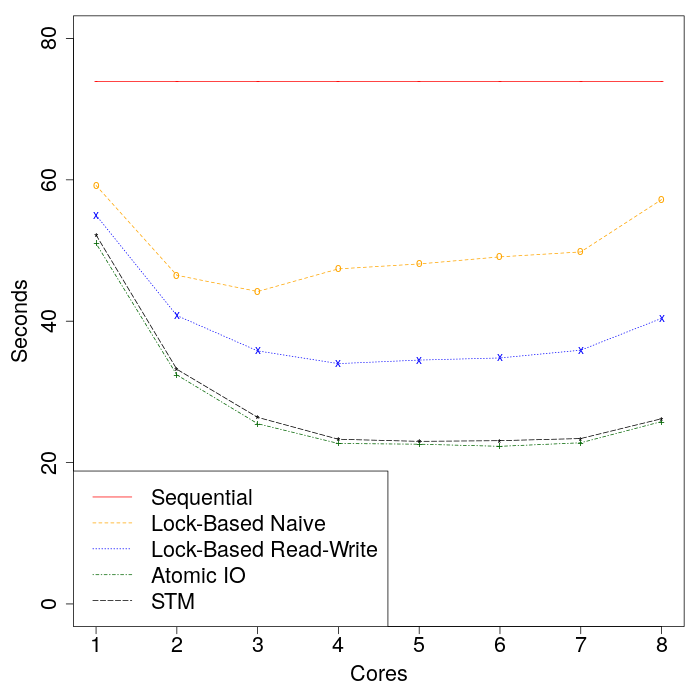
\includegraphics[width=0.8\textwidth, angle=0]{./fig/concurrentabs/sir/sir_varyingcores_constgrid.png}
	\caption{Performance comparison of \textit{Sequential}, \textit{STM}, \textit{Lock-Based} and \textit{Atomic IO} SIR implementations on varying cores with grid size of 51x51 (2,601) agents.}
	\label{fig:sir_varyingcores_constgrid}
\end{figure}

Comparing the performance and scaling to multiple cores of the \textit{STM} and both \textit{Lock-Based} implementations shows that the \textit{STM} implementation significantly outperforms the \textit{Lock-Based} ones and scales better to multiple cores. The \textit{Lock-Based} implementations perform best with 3 and 4 cores respective, and shows decreasing performance beyond 4 cores as can be seen in Figure \ref{fig:sir_varyingcores_constgrid}. This is no surprise because the more cores, the more contention for the central lock, thus the more likely synchronisation happening, ultimately resulting in reduced performance. This is not an issue in \textit{STM} because no locks are taken in advance due to optimistic locking, where a log of changes is kept allowing the runtime to trigger a retry if conflicting changes are detected upon transacting. 

A big surprise however is that the \textit{Atomic IO} implementation is slightly outperforming the \textit{STM} one, which is something we would not have anticipated. We attribute this to the lower overhead of the atomic modification operation.

Both the \textit{STM} and \textit{Atomic IO} implementations are running into decreasing returns after 5 to 6 cores, which we attribute to our hardware. Although virtually it comes across as 8 cores it has only 4 physical ones, implementing hyper threading to simulate 4 additional cores. Due to the fact that resources are shared between two threads of a core, it is only logical that we are running into decreasing returns in all implementations on more than 5 to 6 cores on our hardware.

\subsection{Varying grid size, constant cores}
In this experiment we varied the grid size and used constantly 4 cores. The results are reported in Table \ref{tab:sir_varyinggrid_constcores} and plotted in Figure \ref{fig:sir_varyinggrid_constcores}.

\begin{table}
	\centering
  	\begin{tabular}{ c || c | c | c  }
        Grid Size           & Lock-Based Read-Write & Atomic IO              & STM            \\ \hline \hline 
   		101 x 101 (10,201)  & 139.0 (0.15)          & \textbf{91.1} (0.14)   & 96.5 (0.27)    \\ \hline
   		151 x 151 (22,801)  & 314.0 (0.67)          & \textbf{204.0} (0.36)  & 212.0 (0.16)   \\ \hline
   		201 x 201 (40,401)  & 559.0 (1.22)          & \textbf{360.0} (0.61)  & 382.0 (0.85)   \\ \hline
   		251 x 251 (63,001)  & 861.0 (0.62)          & \textbf{571.0} (0.71)  & 608.0 (1.20)   \\ \hline \hline
  	\end{tabular}

  	\caption{Performance comparison of \textit{Lock-Based Read-Write}, \textit{Atomic IO} and \textit{STM} SIR implementations with varying grid sizes on 4 cores. Timings in seconds (lower is better), standard deviation in parentheses.}
	\label{tab:sir_varyinggrid_constcores} 
\end{table}

It is clear that the \textit{STM} implementation outperforms the \textit{Lock-Based} implementation by a substantial factor. However, the \textit{Atomic IO} implementation outperforms the \textit{STM} one again, where this time the difference is a bit more pronounced due to the higher workload of the experiments. 

\begin{figure}
	\centering
	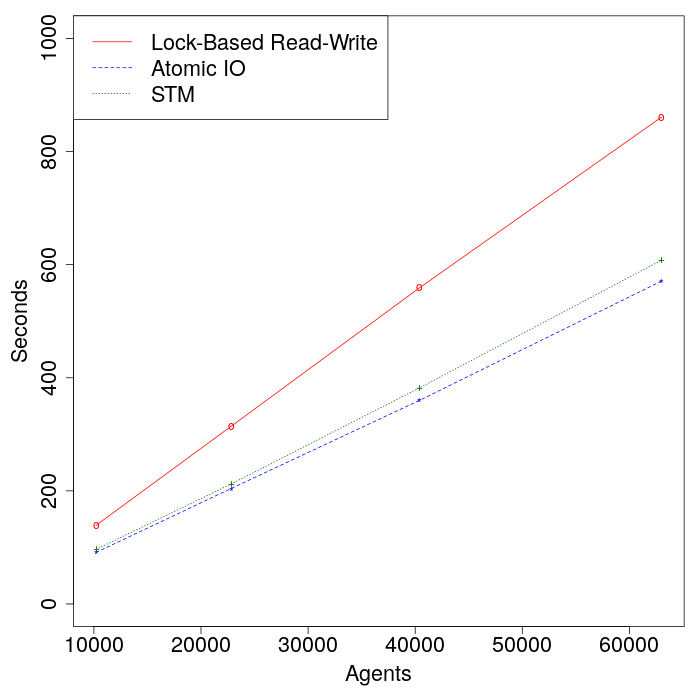
\includegraphics[width=0.8\textwidth, angle=0]{./fig/concurrentabs/sir/sir_varyinggrid_constcores.png}
	\caption{Performance comparison of \textit{Lock-Based Read-Write}, \textit{Atomic IO} and \textit{STM} SIR implementations with varying grid sizes on 4 cores.}
	\label{fig:sir_varyinggrid_constcores}
\end{figure}

\subsection{Retries}
Of very much interest when using STM is the retry ratio, which indicates how many of the total \texttt{STM} actions had to be re-run. A high retry ratio shows that a lot of work is wasted on re-running \texttt{STM} actions due to many concurrent read and writes. Obviously, it is highly dependent on the read-write patterns of the implementation and indicates how well an STM approach is suitable for the problem at hand. We used the \href{http://hackage.haskell.org/package/stm-stats}{stm-stats}~\cite{stm_stats_library} library to record statistics of commits, retries and the ratio. The results are reported in Table \ref{tab:retries_stm}.

\begin{table}
	\centering
  	\begin{tabular}{ c || c | c | c }
        Grid Size 		   & Commits     & Retries  & Ratio  \\ \hline \hline 
   		51 x 51 (2,601)     & 2,601,000   & 1306     & 0.0    \\ \hline
   		101 x 101 (10,201)  & 10,201,000  & 3712     & 0.0    \\ \hline
   		151 x 151 (22,801)  & 22,801,000  & 8189     & 0.0    \\ \hline
   		201 x 201 (40,401)  & 40,401,000  & 13285    & 0.0    \\ \hline
   		251 x 251 (63,001)  & 63,001,000  & 21217    & 0.0    \\ \hline \hline
  	\end{tabular}
  	
  	\caption{Retry ratios of the SIR \textit{STM} implementation with varying grid sizes on 4 cores.}
	\label{tab:retries_stm}
\end{table}

Independent of the number of agents we always have a retry ratio of 0. This indicates that this model is \textit{very} well suited to STM, which is also directly reflected in the much better performance over the \textit{Lock-Based} implementations. Obviously this ratio stems from the fact, that in our implementation we have \textit{very} few conditional writes, which happen only in case when an agent changes from \textit{Susceptible} to \textit{Infected} or from \textit{Infected} to \textit{Recovered}. 

\subsection{Going large scale}
To test how far we can scale up the number of cores in the best performing cases, \textit{Atomic IO} and \textit{STM}, we ran two experiments, 51x51 and 251x251, on an Amazon EC \texttt{m5ad.16xlarge} instance with 16 and 32 cores to see if we are running into decreasing returns. The results are reported in Table \ref{tab:sir_varying_cores_amazon}.

\begin{table}
	\centering
  	\begin{tabular}{cc|c|c}
		\multicolumn{1}{ c||  }{\multirow{2}{*}{} } &
		\multicolumn{1}{ |c| }{Cores} & 51x51    & 251x251       \\ \hline \hline 
		
		\multicolumn{1}{ c||  }{\multirow{2}{*}{Atomic IO} } &
		\multicolumn{1}{ |c| }{16} & 18.0 (0.21)   & 638.0 (8.24)       \\ \cline{2-4}
		\multicolumn{1}{ c||  }{}                       &
		\multicolumn{1}{ |c| }{32} & 15.6 (0.07)   & 720.0 (1.70)      \\ \hline \hline 
		%\multicolumn{1}{ c||  }{}                       &
		%\multicolumn{1}{ |c| }{64} & 28.4 (0.35)   & TODO      \\ \hline \hline 
		
		\multicolumn{1}{ c||  }{\multirow{2}{*}{STM} } &
		\multicolumn{1}{ |c| }{16} & \textbf{14.5} (0.03)  & \textbf{307.0} (1.12)       \\ \cline{2-4}
		\multicolumn{1}{ c||  }{}                          &
		\multicolumn{1}{ |c| }{32} & \textbf{14.7} (0.17)  & \textbf{269.0} (1.05)      \\ \hline \hline 
		%\multicolumn{1}{ c||  }{}                       &
		%\multicolumn{1}{ |c| }{64} & TODO    & TODO      \\ \hline \hline 
	\end{tabular}

  	\caption{Performance comparison of \textit{Atomic IO} and \textit{STM} SIR implementations on 16 and 32 cores on an Amazon EC2 \texttt{m5ad.16xlarge} instance. Timings in seconds (lower is better), standard deviations in parentheses.}
	\label{tab:sir_varying_cores_amazon}
\end{table}

The \textit{Atomic IO} implementation is able to scale up performance from 16 to 32 cores in the case of 51x51 but fails to do so with 251x251. We attribute this behaviour to an increased number of retries of the atomic modification operation, which obviously increases when the number of agents increases. The \textit{STM} implementation performance on the other hand nearly stays constant on 16 and 32 cores in the 51x51 case. In both cases we measured a retry ratio of 0, thus we conclude that with 32 cores we become limited by the overhead of STM transactions \cite{perfumo_limits_2008} because the workload of an STM action in our SIR implementation is quite small. On the other hand, with heavy load as in the 251x251 case, we see an increased performance with 32 cores.

What is interesting is that on more cores, the \textit{STM} implementations has an edge over the \textit{Atomic IO} approach, and performs better in all cases. It seems that for our problem at hand, the atomic modification operation seems to be not as efficient on many cores as an STM approach. 

% NOTE: 0 retries in both cases means that the STM transactions themselves are becoming the bottleneck. this makes sens because the STM trasnactions in our SIR implementation are very small (especially recovered and infected agent) and could therefore really cause substantial overhead as pointed out by \cite{perfumo_limits_2008}
%16 cores 251x251: 0.0 retry ratio
%32 cores 251x251: 0.0 retry ratio
%
%16 cores 51x51: 0.0 retry ratio
%32 cores 51x51: 0.0 retry ratio

\subsection{Summary}
The timing measurements speak a clear language. Running in \texttt{STM} and sharing state using a transactional variable \texttt{TVar} is much more time efficient than the \textit{Sequential} and both \textit{Lock-Based} approaches. On 5 cores \textit{STM} achieves a speedup factor of 3.2 over the \textit{Sequential} implementation, which is a big improvement compared to the simplicity of the approach. What came as a surprise was that the \textit{Atomic IO} approach slightly outperforms the \textit{STM} implementation. However, the \textit{Atomic IO} approach, which uses an atomic modification operation, is only applicable in case there is just a single reference in the program and requires that all operations go through this atomic modification operation. Whether the latter condition is possible or not, is highly dependent on the model semantics, which support it in the case of the SIR model but unfortunately not in the case of Sugarscape.

Obviously both \textit{Lock-Based}, \textit{Atomic IO} and \textit{STM} sacrifice determinism, which means that repeated runs might not lead to same dynamics despite same initial conditions. However, when sticking to STM, we get the guarantee that the source of this nondeterminism is concurrency within the \texttt{STM} Monad but \textit{nothing else}. This can not be guaranteed in the case of both \textit{Lock-Based} and \textit{Atomic IO} approaches as we lose certain static guarantees when running within the \texttt{IO} Monad. The fact to have \textit{both} a substantial speedup \textit{and} the stronger static guarantees, makes the \textit{STM} approach \textit{very} compelling.